Esta etapa tem dois experimentos. O primeiro aumenta o \emph{tamanho} do modelo; o segundo, o \emph{contexto} que ele enxerga. Em cada um, mudamos uma coisa só e mantemos todo o resto igual, para saber a que atribuir a diferença.

\subsection{Experimento 1: um modelo maior}

\paragraph{Pergunta e hipótese.}

O modelo base não teve overfitting e ainda perdia para o 6-grama. Quando treino e validação andam juntos, o modelo provavelmente tem \emph{pouca capacidade} para os dados: ele não consegue nem decorar o treino. A hipótese é que um modelo maior chegue a uma perda menor. Kaplan et al. \cite{kaplan} mediram que, em modelos de linguagem, a perda cai de forma previsível (uma lei de potência) conforme crescem o número de parâmetros, a quantidade de dados e o cálculo gasto no treino.

\paragraph{Montagem do experimento.}

Para a comparação ser justa, mudamos \textbf{só o tamanho} do modelo. Passos, lote, contexto, taxa de aprendizado, dropout e semente ficaram iguais aos da base (\texttt{configs/grande.json}):

\begin{table}[H]
\centering
\begin{tabular}{@{}lcc@{}}
\toprule
 & Base & Grande \\
\midrule
\texttt{n\_embd} ($C$) & 128 & 256 \\
\texttt{n\_head} (dimensão por cabeça) & 4 (32) & 8 (32) \\
\texttt{n\_layer} & 4 & 6 \\
Parâmetros & 833.661 & 4.819.581 (5,8$\times$) \\
Tempo por passo na CPU & $\approx 0{,}15$ s & $\approx 0{,}44$ s \\
Tempo total (5.000 passos) & 12,7 min & 47,6 min \\
\bottomrule
\end{tabular}
\caption{Configurações comparadas. O restante é igual: contexto 64, lote 32, $\eta = 10^{-3}$, dropout 0,1.}
\end{table}

Pela Tabela~\ref{tab:parametros}, cada bloco tem $\approx 12C^2$ parâmetros. Dobrar $C$ multiplica cada bloco por 4, e passar de 4 para 6 blocos multiplica por mais 1,5: daí o fator $\approx 6$.

\paragraph{Resultados.}

Além da estimativa com 100 lotes feita durante o treino, medimos os dois modelos finais no conjunto de validação \emph{inteiro} (508.160 posições), para a comparação com os $n$-gramas ser feita nos mesmos dados:

\begin{table}[H]
\centering
\small
\begin{tabular}{@{}lccccc@{}}
\toprule
Modelo & Perda val. & Bits/caractere & Perplexidade & Treino $-$ val. & Palavras reais \\
\midrule
Unigrama & 3,235 & 4,67 & 25,4 & -- & -- \\
5-grama & 1,223 & 1,76 & 3,40 & -- & -- \\
6-grama & 1,142 & 1,65 & 3,13 & -- & -- \\
Transformer base & 1,249 & 1,80 & 3,49 & $-0{,}029$ & 80\% \\
\textbf{Transformer grande} & \textbf{1,124} & \textbf{1,62} & \textbf{3,08} & $-0{,}036$ & \textbf{87\%} \\
\bottomrule
\end{tabular}
\caption{Validação inteira. ``Treino $-$ val.'' é a diferença no último passo (negativa: o treino vai melhor). Palavras reais: média de 5 amostras a $\tau=0{,}8$, com a mesma semente para os dois modelos (\texttt{compare.py}).}
\label{tab:experimento}
\end{table}

\begin{figure}[H]
\centering
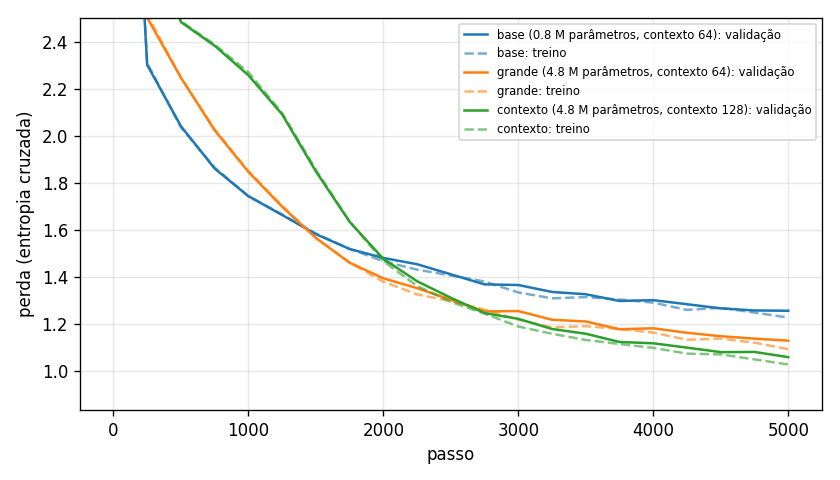
\includegraphics[width=0.8\textwidth]{comparacao.png}
\caption{Curvas de perda dos dois modelos. Linha cheia: validação; tracejada: treino. O eixo vertical foi cortado em 2,5 para mostrar a parte final.}
\label{fig:comparacao}
\end{figure}

\paragraph{Leitura dos resultados.}
\begin{enumerate}
\item \textbf{A hipótese se confirmou.} O modelo grande terminou com perda 0,125 nats menor (1,124 contra 1,249). Em probabilidade média no caractere certo: $e^{-1{,}124} \approx 32{,}5\%$ contra $e^{-1{,}249} \approx 28{,}7\%$.
\item \textbf{O Transformer passou do 6-grama, mas por pouco}: 1,124 contra 1,142. Dois detalhes deixam a comparação ainda mais apertada. A suavização do 6-grama foi escolhida olhando a validação, o que o favorece. Por outro lado, na medição do Transformer, as posições do começo de cada janela de 64 caracteres têm pouco contexto, o que o desfavorece.
\item \textbf{O modelo grande começa mais devagar.} Até o passo $\approx 1.500$, ele fica \emph{acima} da base (Figura~\ref{fig:comparacao}). Com a mesma taxa de aprendizado, um modelo com mais parâmetros precisa de mais passos até organizar suas representações. Depois disso, ele passa a base e a distância só aumenta.
\item \textbf{Com o mesmo tempo de CPU, a base ganha.} Aos 13 minutos, quando a base já tinha terminado com 1,25, o grande estava por volta do passo 1.300, com perda $\approx 1{,}65$. ``Qual modelo é melhor'' depende da pergunta: com o mesmo número de passos, o grande; com o mesmo orçamento de cálculo curto, o pequeno. Hoffmann et al. \cite{hoffmann} estudam exatamente como dividir um orçamento de cálculo entre tamanho do modelo e quantidade de dados.
\item \textbf{O começo de uma separação entre treino e validação.} A diferença final passou de $-0{,}029$ para $-0{,}036$, e no passo 5.000 o treino (1,09) está visivelmente abaixo da validação (1,13). Ainda é pequena, mas é o primeiro sinal de que o modelo maior tem capacidade para começar a decorar. Com mais passos, o dropout e o conjunto de validação passam a ser essenciais.
\item \textbf{Amostras um pouco melhores.} A taxa de palavras reais subiu de 80\% para 87\%. O conteúdo continua sem sentido médico:
\end{enumerate}

\begin{lstlisting}[language={},basicstyle=\ttfamily\footnotesize]
### Revalida 2014
Uma mulher com 44 anos de idade, sem prevenção de mecânio anti-hipertenso. Em
sinais de esclerose impulsiva em espectronente quadro de possa albumina tipa e
pancreática pelo membro inferior de nefrologia à segmentação;
(E) onda endoscopia hormonal do manijor de atenção acessociada a que, está visar
\end{lstlisting}

\begin{atencao}[O que este experimento não mostra]
Fizemos \textbf{um} treino de cada modelo, com \textbf{uma} semente. Parte da diferença pode vir da sorte na inicialização e na ordem dos lotes. Para afirmar com segurança que o grande é melhor, o ideal seria repetir cada treino com 3 sementes e comparar médias e desvios. Aqui, a diferença (0,125 nats) é bem maior que as oscilações entre avaliações vizinhas da mesma curva (cerca de 0,01 a 0,03), o que torna o resultado plausível, mas não o prova.
\end{atencao}

\subsection{Uma correção na forma de medir}

Até aqui, a perda na validação inteira foi medida com janelas de 64 caracteres \emph{lado a lado}. Nelas, o primeiro caractere de cada janela é previsto sem contexto nenhum, o segundo com 1 caractere, e assim por diante: em média, cada previsão usa só 32 caracteres de contexto. Isso subestima o modelo e, pior, torna injusta a comparação entre modelos com contextos diferentes.

A medida correta usa uma \textbf{janela deslizante}: as janelas andam meio contexto por vez e só a segunda metade de cada uma entra na conta. Assim, todo caractere é previsto com pelo menos metade do contexto do modelo. Esse é o método do \texttt{compare.py} a partir daqui. O 6-grama não muda, porque sempre usa os 5 caracteres anteriores.

\begin{table}[H]
\centering
\begin{tabular}{@{}lcc@{}}
\toprule
Modelo & Janelas lado a lado & Janela deslizante \\
\midrule
Transformer base & 1,249 & 1,193 \\
Transformer grande & 1,124 & 1,055 \\
6-grama (referência) & \multicolumn{2}{c}{1,142} \\
\bottomrule
\end{tabular}
\caption{A mesma validação, medida das duas formas. Com a medida correta, o modelo grande passa o 6-grama com folga (1,055 contra 1,142), e não ``por pouco''.}
\end{table}

\subsection{Experimento 2: mais contexto}

\paragraph{Pergunta e hipótese.} As amostras do modelo grande pareciam ``pedaços colados'': cada trecho fazia sentido com a linha anterior, mas o texto perdia o fio. Em 5 amostras de 600 caracteres do modelo grande, medimos que 18\% a 46\% do texto gerado são trechos de 20 ou mais caracteres idênticos ao corpus, mas nenhum passa de 42 caracteres: são as fórmulas das provas (``Assinale a opção que indica''), não questões copiadas. A explicação provável é o contexto de 64 caracteres, cerca de uma linha. A hipótese: com 128 caracteres, o modelo mantém melhor a estrutura da questão.

\paragraph{Montagem.} Igual ao modelo grande, mudando só \texttt{block\_size} de 64 para 128 (\texttt{configs/contexto.json}). A embedding de posição cresce de 64 para 128 linhas, e o modelo passa a ter 4.835.965 parâmetros. Cada passo processa o dobro de caracteres, e o custo da atenção cresce com o quadrado do contexto. O treino levou \textbf{120 minutos} na CPU, contra 48 do grande.

\paragraph{Uma medida de coerência.} Para testar diretamente se o modelo ``lembra'' o que escreveu, contamos, dentro de cada questão gerada, os pares de alternativas seguidas e quantos estão em ordem: \texttt{(A)} depois \texttt{(B)}, \texttt{(B)} depois \texttt{(C)}. Para acertar, o modelo precisa lembrar a letra da alternativa anterior, que muitas vezes está a mais de 64 caracteres de distância. Geramos 90 textos de 1.000 caracteres por modelo, a partir de \texttt{\#\#\# Revalida}, com temperatura 0,8.

\paragraph{Resultados.}

\begin{table}[H]
\centering
\small
\begin{tabular}{@{}lccccc@{}}
\toprule
Modelo & Contexto & Perda (deslizante) & Perplexidade & Alternativas em ordem & Tempo \\
\midrule
6-grama & 5 & 1,142 & 3,13 & -- & -- \\
Base & 64 & 1,193 & 3,30 & -- & 13 min \\
Grande & 64 & 1,055 & 2,87 & 42,7\% (76/178) & 48 min \\
\textbf{Contexto} & \textbf{128} & \textbf{1,015} & \textbf{2,76} & \textbf{74,6\% (94/126)} & 120 min \\
\bottomrule
\end{tabular}
\caption{Os dois experimentos, com a medida correta de perda.}
\label{tab:contexto}
\end{table}

\begin{enumerate}
\item \textbf{A perda caiu de 1,055 para 1,015.} É uma melhora menor que a do Experimento 1, mas vem só do contexto: o número de parâmetros é praticamente o mesmo.
\item \textbf{A coerência melhorou muito}: de 42,7\% para 74,6\% das alternativas em ordem. Um teste de diferença entre duas proporções dá $z \approx 5{,}5$; uma diferença desse tamanho por acaso é praticamente impossível. Esse é o efeito que a perda média esconde: a maioria dos caracteres depende só das letras vizinhas, e o contexto longo importa em poucos pontos, justamente os que dão estrutura ao texto.
\item \textbf{O modelo com mais contexto começa muito mais devagar.} Até o passo $\approx 1.000$, a perda dele fica quase parada entre 2,5 e 2,3, acima dos outros dois. Depois ela cai rápido e passa a do grande por volta do passo 2.750.
\item \textbf{O custo é alto}: 2,5 vezes o tempo do grande, para 0,04 nats a menos. Para um orçamento fixo de tempo, pode valer mais treinar o grande por mais passos.
\end{enumerate}

\subsection{Próximos experimentos sugeridos}

\begin{itemize}
\item \textbf{Treinar o modelo de contexto 128 por mais passos} (10.000 a 15.000), com taxa de aprendizado decrescente, acompanhando a separação entre treino e validação.
\item \textbf{Contexto 256}, idealmente na GPU, já que o custo da atenção cresce com o quadrado do contexto.
\item \textbf{Repetir com sementes diferentes}, para medir a variação entre treinos.
\item \textbf{Treinar na GPU do Kaggle}, que deve ser dezenas de vezes mais rápida que a CPU para esse tamanho de modelo.
\end{itemize}

\begin{exercicios}
\begin{enumerate}
\item Usando $\approx 12C^2$ por bloco, estime os parâmetros de um modelo com $C=384$ e 6 blocos. Quanto tempo por passo você espera na CPU, supondo que o tempo cresce na mesma proporção que os parâmetros?
\item Por que medir no conjunto de validação inteiro é mais confiável que a média de 100 lotes sorteados? Quantas posições cada uma das duas medições usa?
\item Se o treino do modelo grande continuasse até a validação parar de cair, qual checkpoint o \texttt{train.py} guardaria? Por que isso protege contra o overfitting?
\end{enumerate}
\end{exercicios}
